\section{Моделирование применения интерполяции для улучшения характеристик ДН}\label{sect:interpolation-modeling}

Рассмотрим разреженную эквидистантную решётку с межэлементным расстоянием $\lambda/1,4$. 
Для сравнения зададим эквидистантную решётку с межэлементным расстоянием $\lambda/2$. Также для более 
наглядной визуализации сигнала зададим решётку с шагом $\lambda/32$.

\begin{minted}[
    linenos,
    breaklines,
    frame=single,
    framesep=10pt
]{matlab}
f = 5e9; % 5 GHz
lam = freq2wavelen(f); % длина волны
% array params
xmtmin = -0;xmtmax = 12; % начальный и конечный безразмерные координаты элементов эквидистантной решётки с шагом lam/2
dOk = lam/2; % достаточное межэлементное расстояние
dNOk = lam/1.4; % МЭР для разреженной решётки
dSmooth = lam/32; % шаг для сглаживания и визуализации

dxOk = dOk*(xmtmin:1:xmtmax)'; % координаты элементов
NNOk = ceil((max(dxOk)-min(dxOk))/dNOk); % число элементов разреженной решётки
Nsmooth = ceil((max(dxOk)-min(dxOk))/dSmooth); % число элементов решётки для отображения

dxNOk = linspace(min(dxOk),max(dxOk),NNOk)';
dxSmooth = linspace(min(dxOk),max(dxOk),Nsmooth)';
\end{minted}

Если решётка принимает сигнал с направлений близких к направлению на 0~градусов, то значения сигналов не 
сильно отличаются друг от друга, и потому нельзя корректно оценить работу функции интерполяции. 
Проведём начальное исследование с направлением прихода сигнала $\theta=30$~градусов от нормали к плоскости АР. 
Разрешение пространственного отклика АР установим в {0,1}~градус.

\begin{minted}[
    linenos,
    breaklines,
    frame=single,
    framesep=10pt
]{matlab}
aimAngles = [30];
aimAmps   = [0]; %dB
resolution = 0.1; %deg
\end{minted}

Рассмотрим пространственный отклик, полученный для эквидистантных решёток на 
Рисунке~\ref{fig:interpolation-equally-spaced-modeling}.
Наблюдаем главный лепесток на 30~градусах. 
У разреженной решётки также виден дифракционный лепесток на -56~градусах.


\begin{figure}[H]
    \centering
    \begin{subfigure}[b]{0.49\textwidth}
        \centering
        \hspace*{-3ex}
        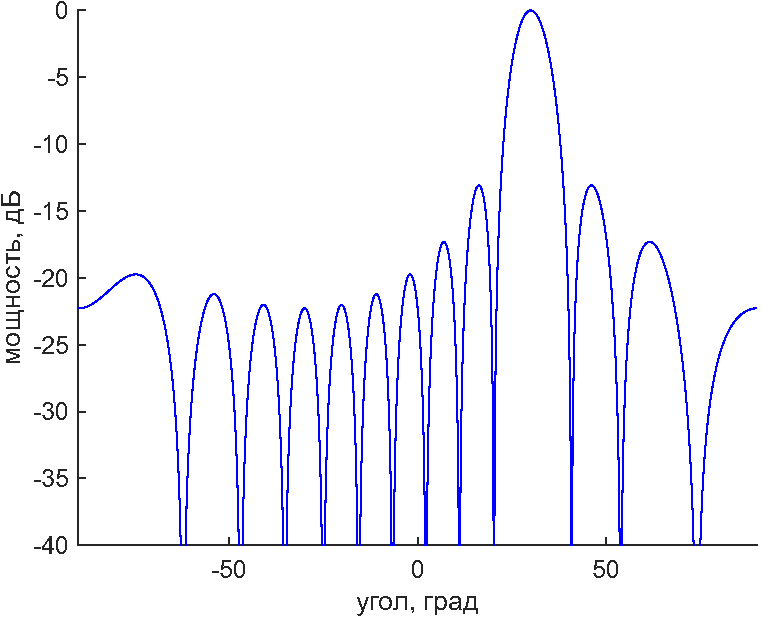
\includegraphics[width=\textwidth]{interpolation-equally-spaced-2}
        \caption{}%
    \end{subfigure}
    \hfill
    \begin{subfigure}[b]{0.49\textwidth}
        \centering
        \hspace*{-3ex}
        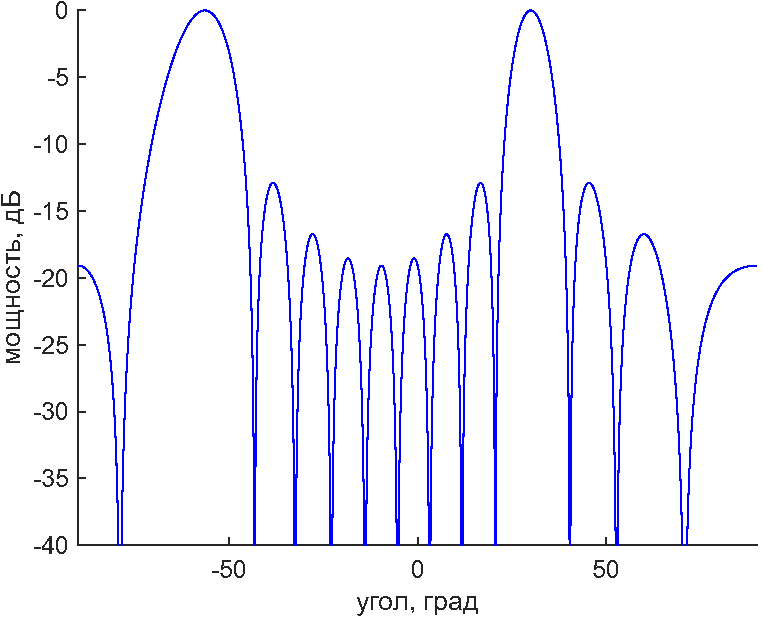
\includegraphics[width=\textwidth]{interpolation-equally-spaced-14}
        \caption{}%
    \end{subfigure}
    \caption{%
    Пространственный отклик эквидистантных решёток с шагом (а) $\lambda/2$ и (б)$\lambda/1,4$
    }%
    \label{fig:interpolation-equally-spaced-modeling}
\end{figure}

Отобразим распределение сигналов для эквидистантных решёток. Также добавим на рисунок графики двух 
сглаженных сигналов, полученных на решётке с шагом $d=\lambda/32$ с направлений +30 и -56~градусов. 
Результат показан на Рисунке~\ref{fig:interpolation-equally-spaced-values}. 

\begin{figure}[H]
    \centering
    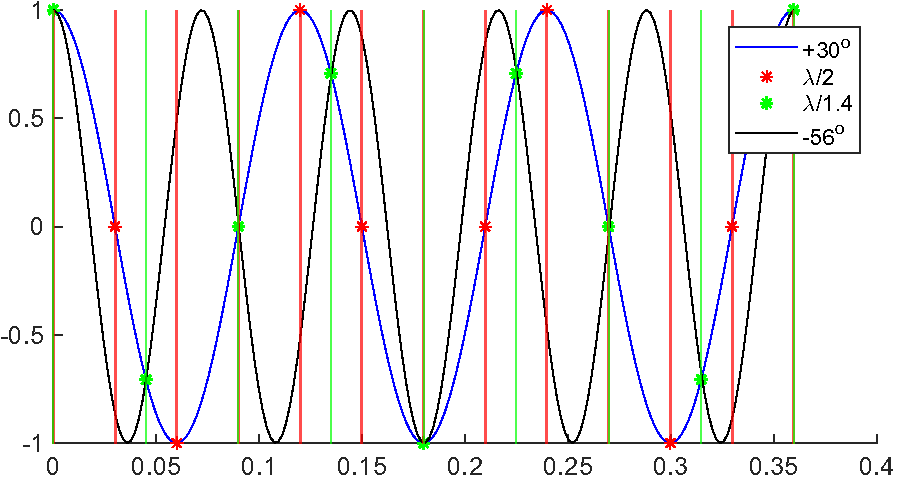
\includegraphics[width=0.8\textwidth]{interpolation-equally-spaced-values}
    \caption{Cравнение распределений для сигналов от целей на +30 и на -56
    градусов от нормали к плоскости антенной решётки}
    \label{fig:interpolation-equally-spaced-values}
\end{figure}

Видно, что значения сигнала на разреженной решётке попадают на пересечения распределений от 
источников на +30 и -56~градусов. Соответственно, в данном случае информация от 
них неотличима, и её не получится использовать для интерполяции.

Создадим ещё одну разреженную решётку с количеством элементов как в эквидистантной разреженной решётке, 
однако с неэквидистантным расположением элементов. При таком расположении элементов информация, 
получаемая при приёме сигналов с различных направлений всегда будет отличаться.

\begin{minted}[
    linenos,
    breaklines,
    frame=single,
    framesep=10pt
]{matlab}
deltas = [0.9 2 1.1 1];
half = cumsum(deltas);
rare2 = dOk*(max(half)+[fliplr(-half),0,half])';
\end{minted}

\begin{figure}[H]
    \centering
    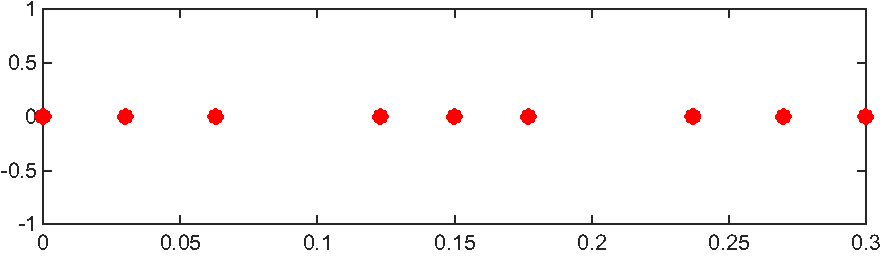
\includegraphics[width=0.8\textwidth]{interpolation-array-pos}
    \caption{Иллюстрация расположения элементов в разреженной решётке}
    \label{fig:interpolation-array-pos}
\end{figure}
    

Расположение выбрано для соответствия поведению функции interp1 из пакета MATLAB: 
Функция interp1 проводит интерполяцию данных в одномерном массиве принимая на вход исходные данные и сетку, 
в которой они расположены, и пересчитывает значения для выходной сетки, используя значения из N ближайших точек 
исходной сетки. 
В данном распределении единичные участки с межэлементным расстоянием $d\gg\lambda/2$ находятся между 
групп элементов с шагом $d\leq \lambda/2$;
значения из узлов с более плотным расположением элементов будут использованы для вычисления значений виртуальных 
элементов в участках с большим межэлементным расстоянием. 

Для неравномерной сетки применимы следующие методы функции interp1:

\begin{itemize}
    \item pchip -- требует минимум 4 точки, кубическая интерполяция
    \item makima -- требует минимум 2 точки, модифицированная кубическая Эрмитова интерполяция
    \item spline -- требует минимум 4 точки, сплайн интерполяция
\end{itemize}

На Рисунке~\ref{fig:interpolation-values-interp-30} показаны результаты интерполяции с применением метода spline. 
Интерполированные данные показаны 
точками синего цвета. Пространственный отклик для интерполированной решётки показан на 
Рисунке~\ref{fig:interpolation-processed-pattern-30}. 
Видно, что при применении интерполяции уровень дифракционных лепестков меньше на {3,5}~дБ по сравнению 
с исходной решёткой без применения интерполяции и на 15~дБ меньше чем в 
эквидистантной разреженной решётке.

\begin{figure}[H]
    \centering
    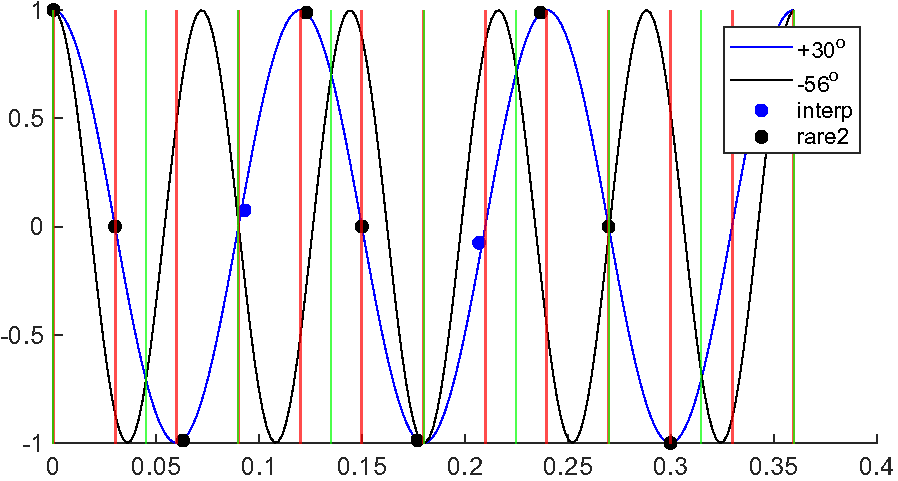
\includegraphics[width=0.8\textwidth]{interpolation-values-interp-30}
    \caption{Сравнение распределений сигналов на различных АР}
    \label{fig:interpolation-values-interp-30}
\end{figure}

\begin{figure}[H]
    \centering
    \begin{subfigure}[b]{0.49\textwidth}
        \centering
        \hspace*{-3ex}
        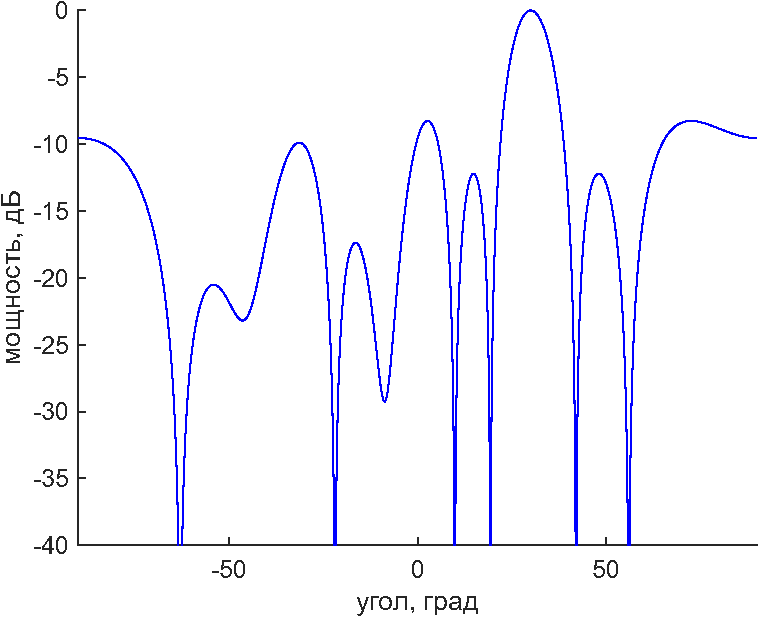
\includegraphics[width=\textwidth]{interpolation-raw-pattern-30}
        \caption{}%
    \end{subfigure}
    \hfill
    \begin{subfigure}[b]{0.49\textwidth}
        \centering
        \hspace*{-3ex}
        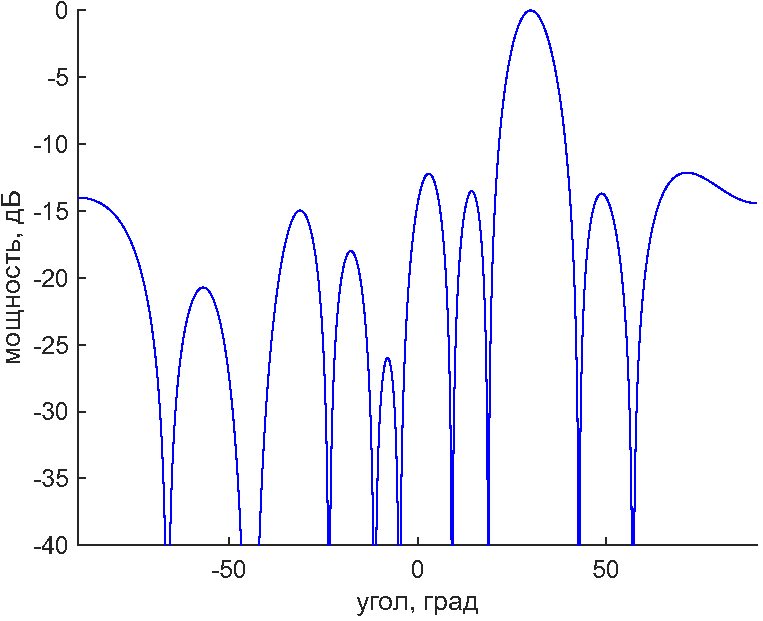
\includegraphics[width=\textwidth]{interpolation-processed-pattern-30}
        \caption{}%
        \label{fig:interpolation-processed-pattern-30}
    \end{subfigure}
    \caption{%
    (а) ДН разреженной решётки
    (б) ДН интерполированной решётки
    }%
    \label{fig:interpolation-pattern-30}
\end{figure}

Проведём ещё одно исследование: увеличим угол отклонения цели от нормального направления до 50 градусов. 
Как видно на Рисунке \ref{fig:interpolation-processed-pattern-50}, применение интерполяции в данном случае 
привело к обратному результату -- в диаграмме направленности лишь усилились нежелательные составляющие. 

\begin{figure}[H]
    \centering
    \begin{subfigure}[b]{0.49\textwidth}
        \centering
        \hspace*{-3ex}
        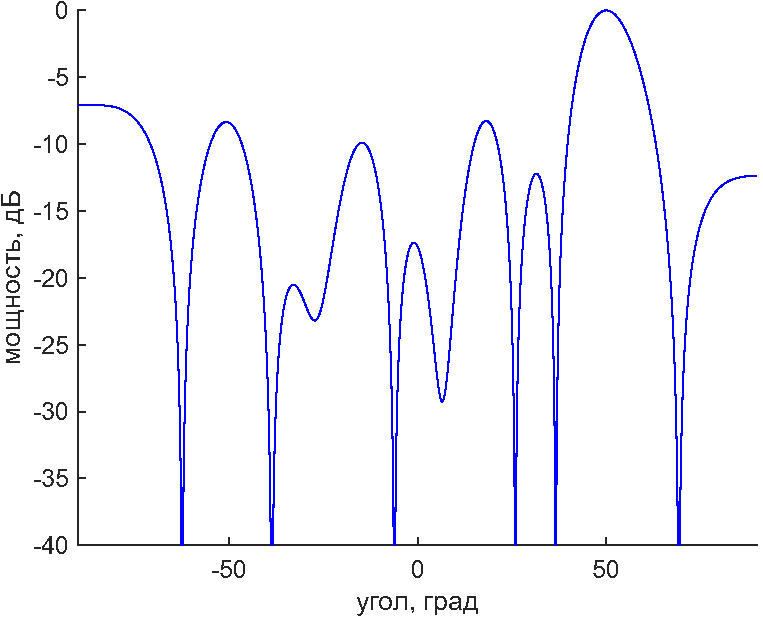
\includegraphics[width=\textwidth]{interpolation-raw-pattern-50}
        \caption{}%
    \end{subfigure}
    \hfill
    \begin{subfigure}[b]{0.49\textwidth}
        \centering
        \hspace*{-3ex}
        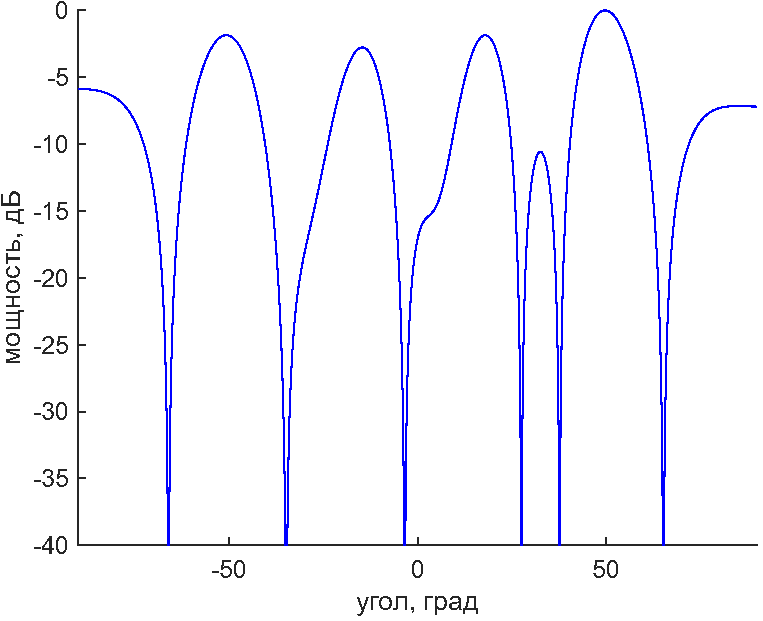
\includegraphics[width=\textwidth]{interpolation-processed-pattern-50}
        \caption{}%
        \label{fig:interpolation-processed-pattern-50}
    \end{subfigure}
    \caption{%
    (а) ДН разреженной решётки
    (б) ДН интерполированной решётки
    }%
    \label{fig:interpolation-pattern-50}
\end{figure}

Рассмотрим распределение сигнала на элементах:

\begin{figure}[H]
    \centering
    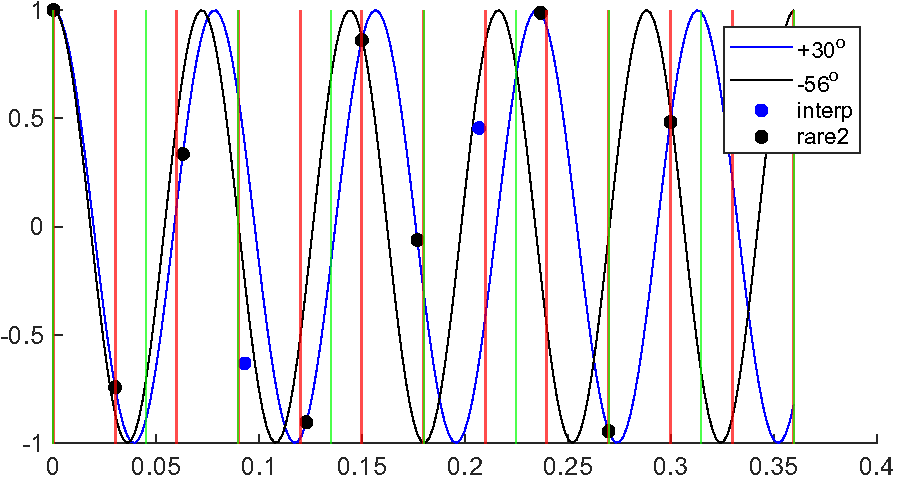
\includegraphics[width=0.8\textwidth]{interpolation-values-interp-50}
    \caption{Сравнение распределений сигналов на различных АР}
    \label{fig:interpolation-values-interp-50}
\end{figure}


Видим, что интерполированные значения сильно отличаются от идеальных т.к. амплитуда колебаний сплайн функции 
меньше амплитуды колебаний синусоидального сигнала. Выбранный метод интерполяции 
плохо подходит для восстановления сигнала. Однако возможно несколько вариантов решения задачи:

\begin{itemize}
    \item Увеличение порядка интерполирующего многочлена для использования большего числа окружающих 
    точек для вычислений, и применение их к АР c большим числом элементов
    \item Применение другого способа интерполяции, учитывающего периодичность сигналов, 
    и использующего все доступные элементы для вычислений каждого значения
\end{itemize}

Оба варианта требуют более глубокого изучения численных методов математического анализа и 
являются темами для дальнейших исследований данного метода.


\subsection{Заключение}

Недостаток данного подхода такой же как у всех других, основанных на применении цифровых антенных решеток, 
а именно -- сложность вычислений. Каждый отсчёт по дальности необходимо дополнительно обрабатывать для 
получения интерполированных распределений, что требует либо применения более производительных центральных процессоров 
либо построения более эффективной параллельной конвейерной архитектуры. Данный недостаток будет всё сильнее проявляться 
с увеличением размера исходной цифровой решётки. В то же время, вычисление значений с помощью интерполяции требует 
меньшего числа операций чем свёртка, которая применяется при поканальной обработке сигнала по дальности. 
Так как данный метод предполагает уменьшение числа элементов антенной решётки, то возможно 
также и уменьшение количества выполняемых операций.

Среди предполагаемых достоинств данного метода можно выделить следующие:

\begin{itemize}
    \item Подавление боковых лепестков - такой подход позволяет добиться меньшего уровня боковых лепестков чем при 
    использовании эквидистантных и неэквидистантных решёток при том же количестве антенных элементов
    \item Экономия средств - как и предыдущий метод, данный позволит уменьшить число антенных элементов по сравнению с 
    эквидистантными ЦАР при схожих параметрах диаграмм направленности.
    \item Выравнивание вычислительной сетки - выходными данными подпрограммы интерполяции являются значения сигналов на 
    виртуальной эквидистантной решётке, что может позволить применять БПФ для ускорения построения ДН, что важно для 
    многолучевых АР и алгоритмов определения направления прихода сигнала. 
\end{itemize}

В целом, стоит отметить, что данный метод выглядит перспективным, однако требует проведения дополнительных исследований. 
Возможно, при использовании данного подхода для каждой конкретной задачи потребуется 
проводить большое количество вычислений для поиска оптимальных распределений для лучших результатов интерполяции. 

